% Template source: University of Florida Department of Physics, https://www.phys.ufl.edu/courses/phy4803L/sample-paper.zip

\documentclass[aps,twocolumn,secnumarabic,nobalancelastpage,amsmath,amssymb,nofootinbib]{revtex4}

% Documentclass Options
    % aps, prl, rmp stand for American Physical Society, Physical Review Letters, and Reviews of Modern Physics, respectively
    % twocolumn permits two columns, of course
    % nobalancelastpage doesn't attempt to equalize the lengths of the two columns on the last page
        % as might be desired in a journal where articles follow one another closely
    % amsmath and amssymb are necessary for the subequations environment among others
    % secnumarabic identifies sections by number to aid electronic review and commentary.
    % nofootinbib forces footnotes to occur on the page where they are first referenced
        % and not in the bibliography
    % REVTeX 4 is a set of macro packages designed to be used with LaTeX 2e.
        % REVTeX is well-suited for preparing manuscripts for submission to APS journals.


\usepackage{chapterbib}    % allows a bibliography for each chapter (each labguide has it's own)
\usepackage{color}         % produces boxes or entire pages with colored backgrounds
\usepackage{graphics}      % standard graphics specifications
\usepackage[pdftex]{graphicx}      % alternative graphics specifications
\usepackage{longtable}     % helps with long table options
\usepackage{epsf}          % old package handles encapsulated post script issues
\usepackage{bm}            % special 'bold-math' package
\usepackage{verbatim}			% for comment environment
\usepackage[colorlinks=true]{hyperref}  % this package should be added after all others
                                        % use as follows: \url{https://urldefense.proofpoint.com/v2/url?u=http-3A__web.mit.edu_8.13&d=DwICAg&c=sJ6xIWYx-zLMB3EPkvcnVg&r=D88uS55Tats-jlFQAC1XryFUYq8B7Lk3StFbXzgsiB4&m=Vjrc9Wj5n5rkIDMPJ5VsRj2GyXC3yXmN_zDHey6dVio&s=_byqsJfgO464rVIugNWFPmbBeIYfNiJcGS1fgIwc0m4&e= }
\usepackage{siunitx}
\usepackage{gensymb}
\usepackage{tikz}

% Graph stuff
% Generated by tikzplotlib
\usepackage[utf8]{inputenc}
\usepackage{pgfplots}
\DeclareUnicodeCharacter{2212}{−}
\usepgfplotslibrary{groupplots,dateplot}
\usetikzlibrary{patterns,shapes.arrows}
\pgfplotsset{compat=newest}

\usetikzlibrary{external}
\tikzexternalize

\usepackage[english]{babel}
\usepackage[autostyle, english=american]{csquotes}
\MakeOuterQuote{"}

%\addtolength\topmargin{-.5\topmargin} %cuts the top margin in half.

%
% And now, begin the document...
% Students should not have to alter anything above this line
%

\begin{document}
\title{Lab 2: Determining the Relationship Between Period and Amplitude}
\author{Tyler Tian}
\date{\today}


\begin{abstract}
TODO: Abstract goes here
\end{abstract}

\maketitle

%%%%%%%%%%%%%%%%%%%%%%%%%%%%%%%%%%%%%%%%%%%%%%%%%%%%%%%%%%%%%%%%%%

\section{Introduction}

TODO: Introduction goes here

%%%%%%%%%%%%%%%%%%%%%%%%%%%%%%%%%%%%%%%%%%%%%%%%%%%%%%%%%%%%%%%%%%

\section{Method}

\subsection{Changes to Data Collection Methods}

As there were no problems identified in the pendulum setup from the last lab, the main structure of the pendulum was
unmodified. However, to accommodate for faster bob velocities, a few changes were made to the rest of the data
collection methods:

\begin{enumerate}
    \item The reflective tape used to marked the pivot was changed into green masking tape. The reflective tape was
          hard to track as it would have a different brightness and colour depending on the viewing and light angle.
          Masking tape allows for more consistent and more accurate tracking due to its uniform colour.
    \item The framerate was increased to 120fps (from 60fps). The larger amplitudes in this lab lead to larger
          velocities and more motion blur, making the tracking less reliable and less accurate. Increasing the framerate
          reduces motion blur and allows for better tracking, leading to smaller time and angle uncertainties.
    \item The light source was changed to a flood light. The previous light source (ceiling light) was not bright or
          focused enough for reliable tracking. A RYOBI ONE+ LED Work Light was used instead of the ceiling light to
          improve tracking.
\end{enumerate}

\begin{figure}[htb]
    \includegraphics[width=0.75\linewidth]{experiment_setup.jpg}
    \caption{The new experiment setup. The red box marks the location of the phone used to record the experiment.}
\end{figure}

The vision tracking program was unmodified (see Appendix \ref{appendix:code}).

\subsection{Data Processing}

To convert from raw time-angle data to amplitude-period data required for this lab, a Python program was used to find
the peaks and valleys of the graph (see Appendix \ref{appendix:code}). Since the data was somewhat noisy, multiple peak
points were averaged to find the time of each peak, and the maximum/minimum of these peak points were taken to find the
peak amplitude.

\begin{figure}[htb]
    % This file was created with tikzplotlib v0.9.15.
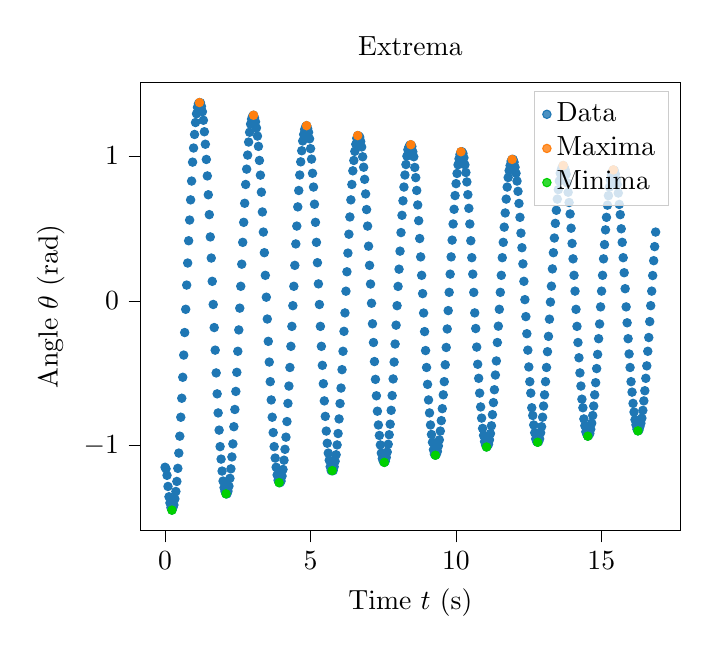
\begin{tikzpicture}

\definecolor{color0}{rgb}{0.12156862745098,0.466666666666667,0.705882352941177}
\definecolor{color1}{rgb}{1,0.498039215686275,0.0549019607843137}

\begin{axis}[
legend cell align={left},
legend style={fill opacity=0.8, draw opacity=1, text opacity=1, draw=white!80!black},
tick align=outside,
tick pos=left,
title={Extrema},
x grid style={white!69.0196078431373!black},
xlabel={Time \(\displaystyle t\) (s)},
xmin=-0.843380281690141, xmax=17.710985915493,
xtick style={color=black},
y grid style={white!69.0196078431373!black},
ylabel={Angle \(\displaystyle \theta\) (rad)},
ymin=-1.58499735593416, ymax=1.50911622481425,
ytick style={color=black}
]
\addplot [draw=color0, fill=color0, mark=*, only marks, mark size=1.5]
table{%
x  y
0 -1.14832393440918
0.0338028169014085 -1.15934008338119
0.0676056338028169 -1.20422093695072
0.101408450704225 -1.28094983688328
0.135211267605634 -1.35212738092095
0.169014084507042 -1.39467415296908
0.202816901408451 -1.42771303312674
0.236619718309859 -1.44435582953651
0.270422535211268 -1.42650693225715
0.304225352112676 -1.40844484488208
0.338028169014085 -1.36677834720235
0.371830985915493 -1.31561393617408
0.405633802816901 -1.24639325872525
0.43943661971831 -1.15598204367384
0.473239436619718 -1.05060528084927
0.507042253521127 -0.933995285246648
0.540845070422535 -0.803147778453946
0.574647887323944 -0.672112827380794
0.608450704225352 -0.52747058376546
0.642253521126761 -0.374333616007584
0.676056338028169 -0.218668945873942
0.709859154929578 -0.0582673029695334
0.743661971830986 0.108812204817245
0.777464788732394 0.261138872382568
0.811267605633803 0.41481428312106
0.845070422535211 0.557708843628792
0.87887323943662 0.696872744673432
0.912676056338028 0.826794618946982
0.946478873239437 0.957336261221193
0.980281690140845 1.05476223569703
1.01408450704225 1.14832393440918
1.04788732394366 1.23057821515021
1.08169014084507 1.29134856266852
1.11549295774648 1.33589796738708
1.14929577464789 1.36028676466754
1.1830985915493 1.36847469841659
1.2169014084507 1.36677834720235
1.25070422535211 1.34210950112267
1.28450704225352 1.30528666800499
1.31830985915493 1.24639325872525
1.35211267605634 1.16700223490976
1.38591549295775 1.08083900054117
1.41971830985916 0.975833278811002
1.45352112676056 0.862170054667226
1.48732394366197 0.732193983853957
1.52112676056338 0.594963047983894
1.55492957746479 0.441179480414981
1.5887323943662 0.29544083714372
1.62253521126761 0.134771284477731
1.65633802816901 -0.0249947936189202
1.69014084507042 -0.184324408899699
1.72394366197183 -0.340218111644683
1.75774647887324 -0.497342716346822
1.79154929577465 -0.64181476975098
1.82535211267606 -0.773493963839138
1.85915492957746 -0.892133836046584
1.89295774647887 -1.00599141735159
1.92676056338028 -1.09216856502672
1.96056338028169 -1.17471488523059
1.9943661971831 -1.2436982297891
2.02816901408451 -1.28902445952154
2.06197183098592 -1.31561393617408
2.09577464788732 -1.33196512721024
2.12957746478873 -1.33196512721024
2.16338028169014 -1.31347261182381
2.19718309859155 -1.2785278441836
2.23098591549296 -1.22492176695766
2.26478873239437 -1.15934008338119
2.29859154929577 -1.07741770401737
2.33239436619718 -0.987423319801041
2.36619718309859 -0.86853939528589
2.4 -0.749699050718124
2.43380281690141 -0.625108534232923
2.46760563380282 -0.493378622777522
2.50140845070423 -0.348060271649564
2.53521126760563 -0.200652877319887
2.56901408450704 -0.0503775071810578
2.60281690140845 0.10050059905463
2.63661971830986 0.253075652164602
2.67042253521127 0.403794091885132
2.70422535211268 0.541846032826459
2.73802816901408 0.673442241654991
2.77183098591549 0.803147778453946
2.8056338028169 0.909024825953549
2.83943661971831 1.00599141735159
2.87323943661972 1.09599676376848
2.90704225352113 1.16369215473891
2.94084507042254 1.21987632938447
2.97464788732394 1.25436487116977
3.00845070422535 1.27291391794195
3.04225352112676 1.28094983688328
3.07605633802817 1.2623783156924
3.10985915492958 1.23571322910411
3.14366197183099 1.19340035955847
3.17746478873239 1.13721484284313
3.2112676056338 1.0661269674222
3.24507042253521 0.968937797100201
3.27887323943662 0.867565685759148
3.31267605633803 0.750118689803857
3.34647887323944 0.613460065573703
3.38028169014085 0.474799563026421
3.41408450704225 0.332332170017718
3.44788732394366 0.17612217382582
3.48169014084507 0.0252047453269417
3.51549295774648 -0.125389120341516
3.54929577464789 -0.279447764126372
3.5830985915493 -0.422472392385715
3.6169014084507 -0.557708843628792
3.65070422535211 -0.683951208097965
3.68450704225352 -0.803147778453946
3.71830985915493 -0.909024825953549
3.75211267605634 -1.00599141735159
3.78591549295775 -1.0847643974548
3.81971830985916 -1.14832393440918
3.85352112676056 -1.20120995242208
3.88732394366197 -1.23846415677718
3.92112676056338 -1.25436487116977
3.95492957746479 -1.25436487116977
3.9887323943662 -1.2436982297891
4.02253521126761 -1.20906708527496
4.05633802816901 -1.16369215473891
4.09014084507042 -1.09963006248179
4.12394366197183 -1.02462976336111
4.15774647887324 -0.940762417248981
4.19154929577465 -0.832981266674432
4.22535211267606 -0.707710521467902
4.25915492957747 -0.588002603547568
4.29295774647887 -0.45990230816097
4.32676056338028 -0.313835152427909
4.36056338028169 -0.17612217382582
4.3943661971831 -0.0333209958782472
4.42816901408451 0.10050059905463
4.46197183098592 0.244978663126864
4.49577464788732 0.392870507464648
4.52957746478873 0.516034091097866
4.56338028169014 0.648534623329675
4.59718309859155 0.761593137212378
4.63098591549296 0.86853939528589
4.66478873239437 0.95937879958371
4.69859154929577 1.03610742281886
4.73239436619718 1.10341739182743
4.76619718309859 1.14832393440918
4.8 1.18247760862243
4.83380281690141 1.20120995242208
4.86760563380282 1.20906708527496
4.90140845070423 1.19028994968253
4.93521126760563 1.16369215473891
4.96901408450704 1.11842643513249
5.00281690140845 1.05060528084927
5.03661971830986 0.978098922059834
5.07042253521127 0.880349869740205
5.10422535211268 0.785398163397448
5.13802816901408 0.666908204239311
5.17183098591549 0.541846032826459
5.2056338028169 0.403794091885132
5.23943661971831 0.263306549569161
5.27323943661972 0.117108744566864
5.30704225352113 -0.0252047453269417
5.34084507042254 -0.17612217382582
5.37464788732394 -0.313835152427909
5.40845070422535 -0.445131206932797
5.44225352112676 -0.57183772991696
5.47605633802817 -0.690446457054692
5.50985915492958 -0.797302362955758
5.54366197183099 -0.898683499414103
5.57746478873239 -0.982793723247329
5.6112676056338 -1.05060528084927
5.64507042253521 -1.09963006248179
5.67887323943662 -1.14486667026095
5.71267605633803 -1.17145387311219
5.74647887323944 -1.17145387311219
5.78028169014085 -1.17145387311219
5.81408450704225 -1.14486667026095
5.84788732394366 -1.10714871779409
5.88169014084507 -1.06206650247934
5.91549295774648 -0.994421106203713
5.94929577464789 -0.915609606361845
5.9830985915493 -0.814975334402692
6.0169014084507 -0.70862627212767
6.05070422535211 -0.601858529694696
6.08450704225352 -0.474799563026421
6.11830985915493 -0.348060271649564
6.15211267605634 -0.210509562127356
6.18591549295775 -0.0831412318884412
6.21971830985916 0.0665681637758238
6.25352112676056 0.200652877319887
6.28732394366197 0.329624407420743
6.32112676056338 0.45990230816097
6.35492957746479 0.578807460409281
6.3887323943662 0.696872744673432
6.42253521126761 0.803147778453946
6.45633802816901 0.897354085139905
6.49014084507042 0.968937797100201
6.52394366197183 1.03181982696575
6.55774647887324 1.08083900054117
6.59154929577465 1.12207298278418
6.62535211267606 1.14071819173903
6.65915492957746 1.13721484284313
6.69295774647887 1.12961684637992
6.72676056338028 1.09963006248179
6.76056338028169 1.06206650247934
6.7943661971831 0.994421106203713
6.82816901408451 0.922261703465222
6.86197183098592 0.838602342940939
6.89577464788732 0.737815060120465
6.92957746478873 0.630033909545915
6.96338028169014 0.516034091097866
6.99718309859155 0.377395967236425
7.03098591549296 0.244978663126864
7.06478873239437 0.11614162687999
7.09859154929577 -0.0165274206027208
7.13239436619718 -0.15832750080843
7.16619718309859 -0.287463205485282
7.2 -0.41906749969982
7.23380281690141 -0.541846032826459
7.26760563380282 -0.655186720433052
7.30140845070423 -0.761593137212378
7.33521126760563 -0.856705628182739
7.36901408450704 -0.928981557043917
7.40281690140845 -0.994421106203713
7.43661971830986 -1.05060528084927
7.47042253521127 -1.08828303177242
7.50422535211268 -1.10714871779409
7.53802816901409 -1.11472433044529
7.57183098591549 -1.10714871779409
7.6056338028169 -1.08083900054117
7.63943661971831 -1.04332574302944
7.67323943661972 -0.989819368774595
7.70704225352113 -0.923899645313353
7.74084507042254 -0.851171414781085
7.77464788732394 -0.75546698504364
7.80845070422535 -0.653635896919522
7.84225352112676 -0.538976499829146
7.87605633802817 -0.422472392385715
7.90985915492958 -0.297882408852949
7.94366197183099 -0.167895923250375
7.97746478873239 -0.0333209958782472
8.0112676056338 0.099668652491162
8.04507042253521 0.218668945873942
8.07887323943662 0.343023940420703
8.11267605633803 0.47116626431311
8.14647887323944 0.590306746935372
8.18028169014084 0.690446457054692
8.21408450704225 0.785398163397448
8.24788732394366 0.86853939528589
8.28169014084507 0.940762417248981
8.31549295774648 0.998958596877937
8.34929577464789 1.04332574302944
8.3830985915493 1.06206650247934
8.41690140845071 1.07345361044807
8.45070422535211 1.07741770401737
8.48450704225352 1.0661269674222
8.51830985915493 1.02895029396844
8.55211267605634 0.994421106203713
8.58591549295775 0.920661816126874
8.61971830985916 0.850395236557051
8.65352112676056 0.761873092412231
8.68732394366197 0.661771500841348
8.72112676056338 0.553294325322293
8.75492957746479 0.430078135055863
8.7887323943662 0.303379917839481
8.82253521126761 0.17612217382582
8.85633802816901 0.0499583957219428
8.89014084507042 -0.0838366420684145
8.92394366197183 -0.212270495716091
8.95774647887324 -0.343023940420703
8.99154929577465 -0.45990230816097
9.02535211267606 -0.576375220591184
9.05915492957747 -0.683951208097965
9.09295774647887 -0.773493963839138
9.12676056338028 -0.856705628182739
9.16056338028169 -0.922261703465222
9.1943661971831 -0.975833278811002
9.22816901408451 -1.02746985796857
9.26197183098592 -1.05794603702369
9.29577464788732 -1.06534798592124
9.32957746478873 -1.05794603702369
9.36338028169014 -1.03907225953609
9.39718309859155 -1.00148313569423
9.43098591549296 -0.95937879958371
9.46478873239437 -0.898683499414103
9.49859154929577 -0.826794618946982
9.53239436619718 -0.744001707847914
9.56619718309859 -0.648534623329675
9.6 -0.557708843628792
9.63380281690141 -0.441179480414981
9.66760563380282 -0.321750554396642
9.70140845070423 -0.194106098030327
9.73521126760564 -0.0671258882021007
9.76901408450704 0.0587558227157227
9.80281690140845 0.184324408899699
9.83661971830986 0.303379917839481
9.87042253521127 0.41906749969982
9.90422535211268 0.530462503588302
9.93802816901409 0.631854380857892
9.97183098591549 0.726642340681726
10.0056338028169 0.808923234382665
10.0394366197183 0.879239376026785
10.0732394366197 0.938941945937004
10.1070422535211 0.980489579859525
10.1408450704225 1.01043644989005
10.1746478873239 1.02895029396844
10.2084507042254 1.02895029396844
10.2422535211268 1.0175020014726
10.2760563380282 0.987423319801041
10.3098591549296 0.938941945937004
10.343661971831 0.885652638903024
10.3774647887324 0.82067763699104
10.4112676056338 0.732815101786507
10.4450704225352 0.638534262219783
10.4788732394366 0.530462503588302
10.512676056338 0.41481428312106
10.5464788732394 0.297882408852949
10.5802816901408 0.184324408899699
10.6140845070423 0.0582673029695334
10.6478873239437 -0.0831412318884412
10.6816901408451 -0.190923158322585
10.7154929577465 -0.319139594272287
10.7492957746479 -0.437631175540433
10.7830985915493 -0.534688903976039
10.8169014084507 -0.636801041548249
10.8507042253521 -0.732193983853957
10.8845070422535 -0.809203189582518
10.9183098591549 -0.880349869740205
10.9521126760563 -0.928981557043917
10.9859154929577 -0.971112011657092
11.0197183098592 -0.994421106203713
11.0535211267606 -1.00860958289487
11.087323943662 -1.00148313569423
11.1211267605634 -0.989819368774595
11.1549295774648 -0.95937879958371
11.1887323943662 -0.915609606361845
11.2225352112676 -0.862170054667226
11.256338028169 -0.785398163397448
11.2901408450704 -0.702256931509007
11.3239436619718 -0.613460065573703
11.3577464788732 -0.511937176307204
11.3915492957746 -0.41481428312106
11.4253521126761 -0.287463205485282
11.4591549295775 -0.17467219900824
11.4929577464789 -0.0582673029695334
11.5267605633803 0.0587558227157227
11.5605633802817 0.17612217382582
11.5943661971831 0.297882408852949
11.6281690140845 0.403794091885132
11.6619718309859 0.508729824315553
11.6957746478873 0.606605108594527
11.7295774647887 0.702256931509007
11.7633802816901 0.785398163397448
11.7971830985915 0.851171414781085
11.830985915493 0.898683499414103
11.8647887323944 0.933995285246648
11.8985915492958 0.96419121820037
11.9323943661972 0.975833278811002
11.9661971830986 0.975833278811002
12 0.957336261221193
12.0338028169014 0.922261703465222
12.0676056338028 0.880349869740205
12.1014084507042 0.826794618946982
12.1352112676056 0.755820992392205
12.169014084507 0.672112827380794
12.2028169014085 0.576375220591184
12.2366197183099 0.467378934967465
12.2704225352113 0.366575389844179
12.3042253521127 0.255182390620818
12.3380281690141 0.134771284477731
12.3718309859155 0.00833314044013592
12.4056338028169 -0.108812204817245
12.4394366197183 -0.226798848053886
12.4732394366197 -0.340218111644683
12.5070422535211 -0.456212801755608
12.5408450704225 -0.557708843628792
12.5746478873239 -0.636801041548249
12.6084507042254 -0.737815060120465
12.6422535211268 -0.791315254103476
12.6760563380282 -0.856705628182739
12.7098591549296 -0.91049007748657
12.743661971831 -0.952499963328554
12.7774647887324 -0.971112011657092
12.8112676056338 -0.975833278811002
12.8450704225352 -0.971112011657092
12.8788732394366 -0.952499963328554
12.912676056338 -0.91049007748657
12.9464788732394 -0.86853939528589
12.9802816901408 -0.803147778453946
13.0140845070423 -0.725944504088791
13.0478873239437 -0.648534623329675
13.0816901408451 -0.557708843628792
13.1154929577465 -0.45990230816097
13.1492957746479 -0.350919997410429
13.1830985915493 -0.244978663126864
13.2169014084507 -0.12644049725839
13.2507042253521 -0.00840316354764699
13.2845070422535 0.101346503265668
13.3183098591549 0.220493761366672
13.3521126760563 0.332332170017718
13.3859154929577 0.433581483951762
13.4197183098592 0.534688903976039
13.4535211267606 0.625108534232923
13.487323943662 0.702256931509007
13.5211267605634 0.767648548340951
13.5549295774648 0.826794618946982
13.5887323943662 0.880349869740205
13.6225352112676 0.903888122555586
13.656338028169 0.922261703465222
13.6901408450704 0.933995285246648
13.7239436619718 0.922261703465222
13.7577464788732 0.903888122555586
13.7915492957746 0.873923582121464
13.8253521126761 0.814975334402692
13.8591549295775 0.749699050718124
13.8929577464789 0.678662490748313
13.9267605633803 0.599684315137805
13.9605633802817 0.50136556146767
13.9943661971831 0.396081441564307
14.0281690140845 0.28984648991162
14.0619718309859 0.17612217382582
14.0957746478873 0.0671258882021007
14.1295774647887 -0.0587558227157227
14.1633802816901 -0.17612217382582
14.1971830985915 -0.287463205485282
14.230985915493 -0.392870507464648
14.2647887323944 -0.497342716346822
14.2985915492958 -0.588002603547568
14.3323943661972 -0.678662490748313
14.3661971830986 -0.737815060120465
14.4 -0.814975334402692
14.4338028169014 -0.862170054667226
14.4676056338028 -0.903888122555586
14.5014084507042 -0.922261703465222
14.5352112676056 -0.933995285246648
14.569014084507 -0.927295218001612
14.6028169014085 -0.915609606361845
14.6366197183099 -0.885652638903024
14.6704225352113 -0.844153986113171
14.7042253521127 -0.791315254103476
14.7380281690141 -0.725944504088791
14.7718309859155 -0.648534623329675
14.8056338028169 -0.564804909443303
14.8394366197183 -0.467378934967465
14.8732394366197 -0.36958637437282
14.9070422535211 -0.261138872382568
14.9408450704225 -0.159646669660662
14.9746478873239 -0.0416425790985884
15.0084507042254 0.0671258882021007
15.0422535211268 0.17612217382582
15.0760563380282 0.28984648991162
15.1098591549296 0.388318718172466
15.143661971831 0.489957326253728
15.1774647887324 0.576375220591184
15.2112676056338 0.660306249308326
15.2450704225352 0.725944504088791
15.2788732394366 0.785398163397448
15.312676056338 0.832981266674432
15.3464788732394 0.86853939528589
15.3802816901408 0.892133836046584
15.4140845070423 0.903888122555586
15.4478873239437 0.898683499414103
15.4816901408451 0.874978137411085
15.5154929577465 0.839238295370751
15.5492957746479 0.803147778453946
15.5830985915493 0.744001707847914
15.6169014084507 0.665494178032424
15.6507042253521 0.594963047983894
15.6845070422535 0.497342716346822
15.7183098591549 0.403794091885132
15.7521126760563 0.297882408852949
15.7859154929577 0.194106098030327
15.8197183098592 0.0838366420684145
15.8535211267606 -0.0416425790985884
15.887323943662 -0.151375443734026
15.9211267605634 -0.261138872382568
15.9549295774648 -0.366575389844179
15.9887323943662 -0.45990230816097
16.0225352112676 -0.557708843628792
16.056338028169 -0.630033909545915
16.0901408450704 -0.707710521467902
16.1239436619718 -0.767436023549591
16.1577464788732 -0.82067763699104
16.1915492957746 -0.855869507976244
16.2253521126761 -0.885652638903024
16.2591549295775 -0.897354085139905
16.2929577464789 -0.892133836046584
16.3267605633803 -0.86853939528589
16.3605633802817 -0.844851822706105
16.3943661971831 -0.809203189582518
16.4281690140845 -0.755820992392205
16.4619718309859 -0.690446457054692
16.4957746478873 -0.620249485982821
16.5295774647887 -0.534688903976039
16.5633802816901 -0.448723344010721
16.5971830985915 -0.348060271649564
16.630985915493 -0.253075652164602
16.6647887323944 -0.143083293668156
16.6985915492958 -0.0333209958782472
16.7323943661972 0.0671258882021007
16.7661971830986 0.17467219900824
16.8 0.277160707333589
16.8338028169014 0.374333616007584
16.8676056338028 0.474799563026421
};
\addlegendentry{Data}
\addplot [draw=color1, fill=color1, mark=*, only marks, mark size=1.5]
table{%
x  y
1.1830985915493 1.36847469841659
3.04225352112676 1.28094983688328
4.86760563380282 1.20906708527496
6.62535211267606 1.14071819173903
8.45070422535211 1.07741770401737
10.1746478873239 1.02895029396844
11.9323943661972 0.975833278811002
13.6901408450704 0.933995285246648
15.4140845070423 0.903888122555586
};
\addlegendentry{Maxima}
\addplot [
  draw=green!81.5686274509804!black,
  fill=green!81.5686274509804!black,
  mark=*,
  only marks, mark size=1.5
]
table{%
x  y
0.236619718309859 -1.44435582953651
2.09577464788732 -1.33196512721024
3.92112676056338 -1.25436487116977
5.74647887323944 -1.17145387311219
7.53802816901409 -1.11472433044529
9.29577464788732 -1.06534798592124
11.0535211267606 -1.00860958289487
12.8112676056338 -0.975833278811002
14.5352112676056 -0.933995285246648
16.2591549295775 -0.897354085139905
};
\addlegendentry{Minima}
\end{axis}

\end{tikzpicture}

    \caption{Zoomed-in view of the first 500 raw data points. The orange and green points are the maxima/minima, from
             which period and amplitude are taken.}
\end{figure}

These are the sources of uncertainty resulting from this method:
\begin{enumerate}
    \item Time (period) uncertainty from the camera: The camera can only capture a set number of frames per second and
          has a nonzero shutter speed. The true peak of an oscillation could lie between two data points, creating an
          uncertainty. An upper bound for this uncertainty can be obtained by taking the time between two frames and
          dividing by 2. At 30 data points per second, this results in an uncertainty of \(\pm 0.02\si{s}\).
          (\textit{Note: while the video was recorded in 120fps to reduce motion blur, the actual rate of data
          collection was only 30 data points/second.})
    \item Period uncertainty from noise in the data and inaccuracies in peak finding: Due to noise in the data,
          sometimes the true peak location is not apparent. The code attempts to correct this by taking the mean of all
          peak candidates. The standard deviation of the time values of the peak candidates is used as the uncertainty,
          and experimentally determined to be about \(\pm 0.06\si{s}\).
    \item Amplitude uncertainty caused by the previous two uncertainties: Since the true peak may lie between two data
          points (as per \textcircled{1}) and is influenced by noise (as per \textcircled{2}), this creates an
          uncertainty. As the exact value of this uncertainty is hard to find, it is assumed to be the same in
          percentage as the larger of the two sources above.
    \item Amplitude uncertainty caused by the decay of the pendulum over one oscillation: The pendulum's amplitude
          decays as it swings, creating an uncertainty. By substituting $t = T$ into the pendulum equation, we obtain
          an exponential term of $e^{-\frac{T}{t}} = e^{-\frac{\pi}{Q}}$. In other words, the amplitude decays by a
          factor of $e^{-\frac{\pi}{Q}}$ per oscillation. The relative change in amplitude is then
          $1 - e^{-\frac{\pi}{Q}}$; by substituting in the $Q$ value obtained in the previous lab (about 140), the
          amount of decay is found to be $2.2\%$, so the uncertainty is \(\pm 2\%\).
\end{enumerate}

Additionally, there may be an amplitude uncertainty resulting from imperfect computer vision tracking, but due to the
improved setup, this can be assumed to be much less than the other sources listed above.

\subsection{Data Fitting}

%%%%%%%%%%%%%%%%%%%%%%%%%%%%%%%%%%%%%%%%%%%%%%%%%%%%%%%%%%%%%%%%%%

\section{Observations}

TODO: Observations here

%%%%%%%%%%%%%%%%%%%%%%%%%%%%%%%%%%%%%%%%%%%%%%%%%%%%%%%%%%%%%%%%%%

\section{Analysis and Conclusion}

TODO: Analysis here

%%%%%%%%%%%%%%%%%%%%%%%%%%%%%%%%%%%%%%%%%%%%%%%%%%%%%%%%%%%%%%%%%%

\appendix

\section{Source Code}

A comprehensive list of all source code, as well as the \LaTeX{} source for this report, can be found on GitHub at
\url{https://github.com/tylertian123/phys180_lab}, in particular:
\label{appendix:code}
\begin{enumerate}
    \item List individual items here
\end{enumerate}

\end{document}
